\documentclass[11pt]{article}
\usepackage[utf8]{inputenc}
\usepackage[T1]{fontenc}
\usepackage{amsmath}
\usepackage{multicol}
\usepackage{geometry}
\usepackage{tikz}
\usetikzlibrary{shapes.geometric, arrows.meta}
\usepackage{enumitem}
\usepackage{xcolor}
\usepackage{titlesec}

% Configurações de layout
\geometry{a4paper, left=1cm, right=1cm, top=0.5cm, bottom=1.2cm}
\setlength{\columnseprule}{0.4pt}
\setlength{\baselineskip}{1.0\baselineskip}

% Cores para títulos
\titleformat{\section}{\normalfont\Large\bfseries\color{blue}}{\thesection}{1em}{}
\titleformat{\subsection}{\normalfont\large\bfseries\color{red}}{\thesubsection}{1em}{}
\titleformat{\subsubsection}{\normalfont\normalsize\bfseries\color{black}}{\thesubsubsection}{1em}{}

\title{\textcolor{blue}{Função do 1º Grau: Conceitos e Aplicações}}
\author{Professor: Jefferson}
\date{}

\begin{document}

\maketitle
\vspace{-1cm}

\begin{center}
\large{Nome: \underline{\hspace{8cm}} \quad Turma: \underline{\hspace{3cm}}}
\end{center}

\begin{multicols}{2}

\section*{1. Conceito}
Uma função do 1º grau (ou função afim) é uma relação matemática expressa por:
\[
f(x) = ax + b \quad \text{ou} \quad y = ax + b
\]
onde:
\begin{itemize}
    \item $a$ é o coeficiente angular (inclinação da reta)
    \item $b$ é o coeficiente linear (ponto onde a reta corta o eixo y)
    \item $x$ é a variável independente
    \item $f(x)$ ou $y$ é a variável dependente
\end{itemize}

\subsection*{Exemplos}
\begin{itemize}
    \item $f(x) = 2x + 1$ \quad ($a=2$, $b=1$)
    \item $y = -x + 3$ \quad ($a=-1$, $b=3$)
    \item $f(x) = \frac{1}{2}x - 4$ \quad ($a=\frac{1}{2}$, $b=-4$)
\end{itemize}

\section*{2. Gráfico}
O gráfico de uma função do 1º grau é sempre uma \textbf{reta}. Para construí-lo:

\begin{enumerate}
    \item Encontre dois pontos quaisquer
    \item Marque-os no plano cartesiano
    \item Trace a reta que passa por eles
\end{enumerate}

\begin{center}
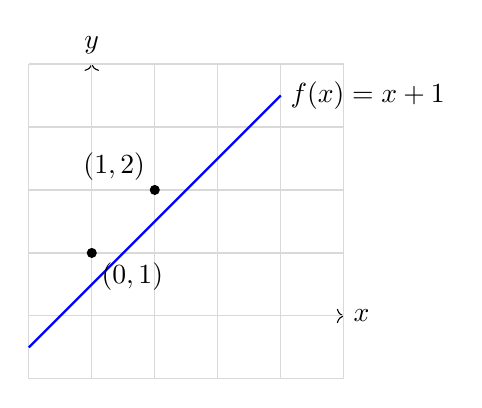
\begin{tikzpicture}[scale=0.8]
    % Eixos
    \draw[->] (-1,0) -- (4,0) node[right]{$x$};
    \draw[->] (0,-1) -- (0,4) node[above]{$y$};
    % Grade
    \draw[gray!30] (-1,-1) grid (4,4);
    % Função f(x) = x + 1
    \draw[blue, thick] (-1,-0.5) -- (3,3.5);
    \node at (3,3.5) [right] {$f(x)=x+1$};
    % Pontos
    \filldraw (0,1) circle (2pt) node[below right]{$(0,1)$};
    \filldraw (1,2) circle (2pt) node[above left]{$(1,2)$};
\end{tikzpicture}
\end{center}

\section*{3. Coeficientes}
\subsection*{Coeficiente Angular ($a$)}
\begin{itemize}
    \item Determina a \textbf{inclinação} da reta
    \item Calculado por: $a = \frac{\Delta y}{\Delta x} = \frac{y_2-y_1}{x_2-x_1}$
    \item Se $a > 0$: função crescente
    \item Se $a < 0$: função decrescente
\end{itemize}

\subsection*{Coeficiente Linear ($b$)}
\begin{itemize}
    \item Ponto onde a reta corta o eixo $y$
    \item Corresponde ao valor de $f(0)$
\end{itemize}

\begin{center}
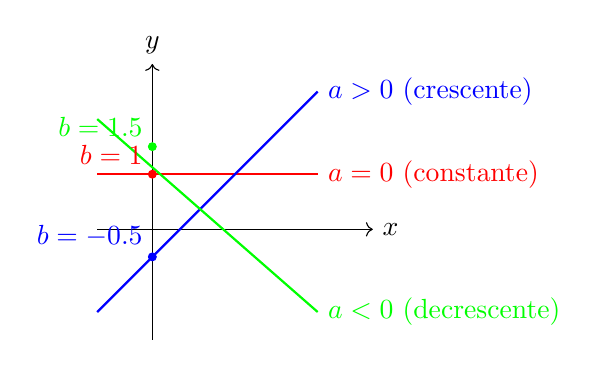
\begin{tikzpicture}[scale=0.7]
    % Eixos
    \draw[->] (-1,0) -- (4,0) node[right]{$x$};
    \draw[->] (0,-2) -- (0,3) node[above]{$y$};
    % Funções
    \draw[red, thick] (-1,1) -- (3,1) node[right]{$a=0$ (constante)};
    \draw[blue, thick] (-1,-1.5) -- (3,2.5) node[right]{$a>0$ (crescente)};
    \draw[green, thick] (-1,2) -- (3,-1.5) node[right]{$a<0$ (decrescente)};
    % b
    \filldraw[red] (0,1) circle (2pt) node[above left]{$b=1$};
    \filldraw[blue] (0,-0.5) circle (2pt) node[above left]{$b=-0.5$};
    \filldraw[green] (0,1.5) circle (2pt) node[above left]{$b=1.5$};
\end{tikzpicture}
\end{center}

\section*{4. Zero da Função (Raiz)}
O zero da função é o valor de $x$ que torna $f(x) = 0$:
\[
ax + b = 0 \Rightarrow x = -\frac{b}{a}
\]
É o ponto onde a reta corta o eixo $x$.

\subsection*{Exemplo}
Para $f(x) = 2x - 4$:
\[
2x - 4 = 0 \Rightarrow x = 2
\]

\begin{center}
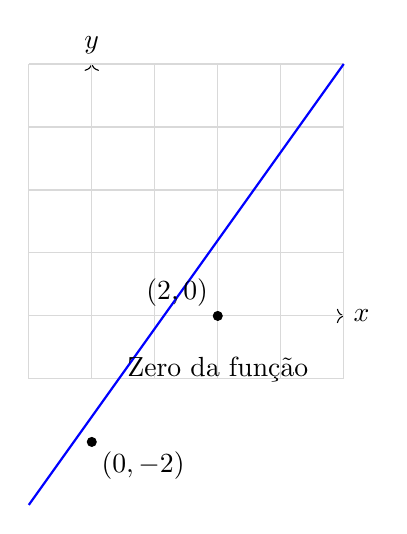
\begin{tikzpicture}[scale=0.8]
    % Eixos
    \draw[->] (-1,0) -- (4,0) node[right]{$x$};
    \draw[->] (0,-1) -- (0,4) node[above]{$y$};
    % Grade
    \draw[gray!30] (-1,-1) grid (4,4);
    % Função
    \draw[blue, thick] (-1,-6/2) -- (4,4);
    % Pontos
    \filldraw (0,-2) circle (2pt) node[below right]{$(0,-2)$};
    \filldraw (2,0) circle (2pt) node[above left]{$(2,0)$};
    % Zero
    \node at (2,-0.5) [below] {Zero da função};
\end{tikzpicture}
\end{center}

\section*{5. Estudo do Sinal}
\begin{itemize}
    \item $f(x) > 0$ para valores de $x$ acima da raiz (se $a>0$) ou abaixo (se $a<0$)
    \item $f(x) < 0$ para valores de $x$ abaixo da raiz (se $a>0$) ou acima (se $a<0$)
\end{itemize}

\begin{center}
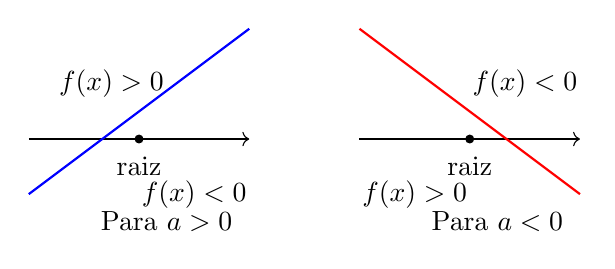
\begin{tikzpicture}[scale=0.7]
    % Caso a>0
    \draw[->] (-1,0) -- (3,0);
    \draw[blue, thick] (-1,-1) -- (3,2);
    \filldraw (1,0) circle (2pt);
    \node at (1,-0.5) {raiz};
    \node at (0.5,1) {$f(x)>0$};
    \node at (2,-1) {$f(x)<0$};
    \node at (1.5,-1.5) {Para $a>0$};
    
    % Caso a<0
    \draw[->] (5,0) -- (9,0);
    \draw[red, thick] (5,2) -- (9,-1);
    \filldraw (7,0) circle (2pt);
    \node at (7,-0.5) {raiz};
    \node at (6,-1) {$f(x)>0$};
    \node at (8,1) {$f(x)<0$};
    \node at (7.5,-1.5) {Para $a<0$};
\end{tikzpicture}
\end{center}

\section*{6. Aplicações Práticas}
\subsection*{Exemplo 1: Taxa de Serviço}
Um técnico cobra R\$ 50,00 de visita mais R\$ 30,00 por hora de trabalho. A função que representa o custo $C$ em relação às horas $h$ é:
\[
C(h) = 30h + 50
\]

\subsection*{Exemplo 2: Vendas}
Um vendedor tem salário composto por R\$ 800,00 fixos mais R\$ 2,00 por item vendido. A função salário $S$ em relação aos itens $v$ é:
\[
S(v) = 2v + 800
\]

\section*{Exercícios Básicos (1-10)}
\begin{enumerate}
    \item Dada \( f(x) = 3x - 6 \), determine:
    \begin{enumerate}[label=\alph*)]
        \item Coeficiente angular
        \item Coeficiente linear
        \item Zero da função
    \end{enumerate}
    
    \item Classifique como crescente ou decrescente:
    \begin{enumerate}[label=\alph*)]
        \item \( y = 5x - 2 \)
        \item \( f(x) = -x + 4 \)
    \end{enumerate}
    
    \item Calcule \( f(2) \) para:
    \begin{enumerate}[label=\alph*)]
        \item \( f(x) = 4x - 3 \)
        \item \( f(x) = -2x + 5 \)
    \end{enumerate}
    
    \item Encontre o ponto onde corta o eixo y:
    \begin{enumerate}[label=\alph*)]
        \item \( y = \frac{1}{2}x + 3 \)
        \item \( f(x) = -3x - 1 \)
    \end{enumerate}
    
    \item Determine a função que passa por:
    \begin{enumerate}[label=\alph*)]
        \item \( (0,2) \) e \( (1,5) \)
        \item \( (2,4) \) e \( (3,1) \)
    \end{enumerate}
\end{enumerate}

\section*{Exercícios Intermediários (11-20)}
\begin{enumerate}\setcounter{enumi}{5}
    \item Construa os gráficos de:
    \begin{enumerate}[label=\alph*)]
        \item \( y = 2x - 4 \)
        \item \( f(x) = -x + 3 \)
    \end{enumerate}
    
    \item Resolva:
    \begin{enumerate}[label=\alph*)]
        \item Se \( f(x+1) = 3x - 2 \), encontre \( f(4) \)
        \item Se \( f(2) = 7 \) e \( f(5) = 13 \), determine \( f(x) \)
    \end{enumerate}
    
    \item Aplicações:
    \begin{enumerate}[label=\alph*)]
        \item Um táxi cobra R\$ 5,00 de bandeirada mais R\$ 2,80/km. Escreva \( C(x) \)
        \item Calcule o custo para 15 km
    \end{enumerate}
    
    \item Estude o sinal:
    \begin{enumerate}[label=\alph*)]
        \item \( f(x) = 6x - 12 \)
        \item \( y = -4x + 8 \)
    \end{enumerate}
    
    \item Problemas:
    \begin{enumerate}[label=\alph*)]
        \item Uma empresa tem custo fixo R\$ 1.200,00 e custo variável R\$ 8/unidade. Escreva \( C(x) \)
        \item Se vende por R\$ 15/unidade, qual o lucro para 300 unidades?
    \end{enumerate}
\end{enumerate}

\section*{Exercícios Avançados (21-30)}
\begin{enumerate}\setcounter{enumi}{10}
    \item Determine \( k \) para que:
    \begin{enumerate}[label=\alph*)]
        \item \( f(x) = (k-2)x + 5 \) seja crescente
        \item \( f(x) = (3k+1)x - 4 \) seja decrescente
    \end{enumerate}
    
    \item Verifique se pertence à função:
    \begin{enumerate}[label=\alph*)]
        \item \( (3,10) \) pertence a \( y = 4x - 2 \)?
        \item \( (-2,-7) \) pertence a \( f(x) = 3x - 1 \)?
    \end{enumerate}
    
    \item Sistemas:
    \begin{enumerate}[label=\alph*)]
        \item Em qual ponto \( y = 2x - 3 \) intercepta \( y = -x + 6 \)?
        \item Resolva o sistema: \( \begin{cases} y = 3x - 4 \\ y = -2x + 6 \end{cases} \)
    \end{enumerate}
    
    \item Funções definidas por partes:
    \begin{enumerate}[label=\alph*)]
        \item Dada \( f(x) = \begin{cases} 2x+1, & \text{se } x \geq 0 \\ -x+3, & \text{se } x < 0 \end{cases} \), calcule \( f(2) \) e \( f(-1) \)
    \end{enumerate}
    
    \item Problemas complexos:
    \begin{enumerate}[label=\alph*)]
        \item Um celular custa R\$ 1.200,00 à vista ou R\$ 200,00 de entrada mais 12 parcelas de R\$ 90,00. Em quantos meses a compra a prazo iguala o valor à vista?
        \item Dois táxis têm modelos: Taxi A: R\$ 4,00 bandeirada + R\$ 2,50/km; Taxi B: R\$ 3,00 bandeirada + R\$ 2,80/km. A partir de quantos km o Taxi A fica mais barato?
    \end{enumerate}
\end{enumerate}

\end{multicols}

\end{document}
